%
% ---------------------------------------------------
%
% Trabajo de Final de Grado:
% Author: Gonzalo Jesús García Martín <dracoyue@gmail.com>
% Capítulo: Objetivos
% Fichero: Cap10_Presupuesto.tex
%
% ----------------------------------------------------
%

\cleardoublepage
\chapter{Presupuesto}
\label{chap:budget}

	Este presupuesto está dirigido a empresas, principalmente a colegios que deseen adquirir \CollegeApp. Se ha desglosado en el presupuesto la cantidad de horas de análisis y de implementación que se han empleado en cada funcionalidad de la aplicación.
		
		\begin{figure}[h !]
			\centering
			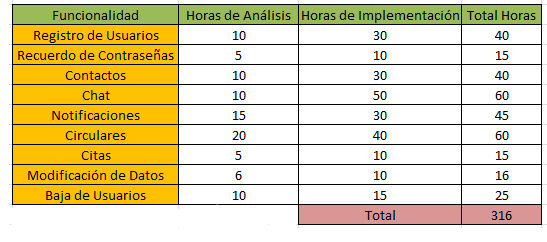
\includegraphics{horas}
			\caption{Horas empleadas en el desarrollo de la aplicación}
			\label{fig:presupuesto}
		\end{figure}
		
		La cantidad de horas invertidas en la aplicación son {\bf 316 horas}. La tarifa de desarrollo establecida en este proyecto es de {\bf 3.5 euros la hora} lo cual conduce a un total de {\bf 1106 euros de honorarios}. A lo cual hay que agregarle la adquisición de dos dispositivos de gama media a {\bf 119 euros cada uno} para pruebas con la aplicación.
		
		\bigskip
		Dicho esto, la aplicación tiene un coste de {\bf \large 1334 euros}.